\chapter{Materials and Methods}\label{chap:MaterialsAndMethods}
	\section{Low field NMR}
		To achieve NMR spectra at fields where SABRE is feasible \todo{Ref sabre}, a low field NMR
		spectrometer was built \todo{ref niels}. Its main field is genrated by a resisitve solenoid
		coil. Inside that coil, there is a saddle coil
		generating a $B_1$ field perpendicular to $B_0$. Perpendicular to and inside both, a third
		coil, also a solenoid, is used to detect the signal generated by the spins.
		\subsection{Static Magnetic Field}
			The $B_0$ coil is wound around an acrylic tube in two full layers. In addition, at the
			tube's ends compensation windings are installed to homogenize the field inside the coil.
			The length of these windings was optimized in matlab simulations \todo{figure of whole setup}
		\subsection{Radiofrequency Excitation}
			To irradiate samples with radiofrequency pulses, a saddle coil \todo{dimensions} wsa
			used. It was operated untuned and unmatched as a broadband resonator. The pulse
			generation was performed using a National Instruments data acquisition crate (NI
			\todo{which?}). 
		\subsection{Software control}
			All software control was realized using Matlab in combination with the DAQmx libraries.
			The prevoiusly existing code was strongly modified in the course of this work to
			implement more features and fix buggy behaviour.
		\subsection{Data Readout}
			All readout was done using a 12 bit NI \todo{name} card operating 10 MS/s. The signal
			was recorded directly without preamplification or mixing. That required small distances
			between readout coil and NI card to keep signal losses at bay. 
		\subsection{Shim System}
			For homogenization of the field, a shim system was built according to Biot Savart
			simulations. It features linear shim coils for all three spatial dimensions mounted to a
			.\todo{cm} acrylic tube. The x and y shims are made of four saddle coils respectively that
			were plainly manufactured individually and bent to fit the tube. The z shims, which are
			basically a pair of maxwell coils, were added on top of these saddle coils. All shims
			are driven by a \todo{H\&U} programmable power supply providing up to
			$\SI{10}{\ampere}$ of current. The power supply is connected via a virtual serial port inside
			a USB connection. That way, the three shim channels can be controlled from inside the
			Matlab hypercontrol program \ref{subsec:hypercontrol}
	\section{Magritek Low Field MRI}
		To acquire images at low fields, a Magritek Terranova \todo{ref } was used. It features
		similar hardware as the low field spectrometer, but uses its $B_0$ coil only for
		prepolarization while signal is acquired at Earth magnetic field.
		%\subsection{
		\todo{subsections}
	\section{Bruker Low Field MRI}
		\subsection{Gradient Coil Setup}
		\subsection{Signal mixer}
		\subsection{Receive coil}
		\subsection{Paravision and Topspin software}
	\section{High field MRI}
		The most well known application of NMR is the high field MRI of human antomy with its
		widespread use in clinics around the world. Not as common, but equally important are
		preclinical scanners for research purposes. These preclinical scanner, primarily built for
		animal experiments, were used in most of the high field experiments shown in this work.
		\subsection{MRI Hardware}
			For the acquisition of spectra and images, hardware for different purposes is requred:
			\begin{itemize}
			\item $B_0$ field generation
			\item Pulse generation
			\item Field gradients generation
			\item Signal readout
			\end{itemize}
		\subsection{Paravision Software}
			The stadard Bruker imaging software called paravision features sequence and method
			implementations for the more common use cases and can additionally be modified for
			specific purposes. Sequence programming is generally in C++ while many other
			modifications can be done via GUIs.
			For the purposes of this work, the most common sequences were rather simplistic NMR
			sequences while some images of hyperpolarized tracers have been generated with more
			sophisticated imaging sequences.
		\subsection{Custom High Field Coils}
			Most commercially available coils are for proton imaging and spectroscopy. Coils for
			other nuclei are obtainable, but usually expensive and not necessarily tailored to the
			specific purpose in mind. Therefore, we built single and dual tune coils for different
			nuclei and different fields.
			\subsubsection{$^{15}N$ coil}
				A solenoid of thick, stable copper wire was wound to fit the experimental setup of
				the shuttling system described in \ref{sec:shuttlingSystem}. The solenoid was
				attached to a circuit board via clamped and soldered connections. On the board, a
				high voltage tune capacitor as well as two symmetric matching capacitors were
				installed. Coaxial cable was used to make the connection to the scanner and the
				whole setup was mounted to a teflon holder for precise positioning.
				The tune capacitor was chosen so that it can be tuned to both a $\SI{7}{\tesla}$ and
				a $\SI{9.4}{\tesla}$ field at $\SI{300}{\MHz}$ and $\SI{400}{\MHz}$ respectively.
				\todo{image coil}
				
	\section{Shuttling system}\label{sec:shuttlingSystem}
		To measure in-situ Sabre polarized substances at high fields, a transfer system is
		necessary. This system can either move a probe inside a closed container
		\ref{setupNovosibirsk} or transfer the probe itself via tubings. We chose the latter for the
		more flexible and less difficult positioning especially in the environment of a lieing bore
		small animal scanner as compared to a standing bore spectrometer. In addition, all actuation
		can be done by non-magnetic gases which was beneficial especially at the $\SI{9.4}{\tesla}$
		machine which is unshielded and creates $\SI{5}{\gauss}$ fields in a distance of about $\SI{1}{\meter}$ from
		the scanner bore.
		\subsection{Magnetic Shielding}
			To be able to polarize $^{15}N$ using Sabre Sheath \ref{}, fields of the order of
			magnitude of $\SI{100}{\nano\tesla}$ were necessary. Thus, Earth magnetic field needed to
			be shielded against. To do so, we purchased a three-layered Mu-Metal shield (ZG-218, Magnetic
			Shield Corp.) with shielding factors of 100 per layer.
		\subsection{Low Field Reactor}
			At low field, multiple design features have to be combined to achieve high polarization
			yields. First off, pH2 has to be supplied to the sample continuously and efficiently.
			Positioning of the probe has to be reproducible to ensure the fields are well defined.
			The system must be resistant to the chemicals and solvents used in the experiments and
			hold the pressures applied during measurements. Furthermore, it must be non magnetic to
			not distort residual fields inside the shield which otherwise might reduce polarization
			in parts of the sample. To fulfill all these requirements, polysulphone (PSU) was chosen
			as a material because of its high mechanical and chemical stability. The reactor was
			designed in Inventor (Autodesk) as a body of rotation. It features a sample volume of
			about $\SI{3}{\mm\cubed}$ with a larger diameter venting area to reduce sample losses
			due to foaming and spray. Below the sample volume, a interchangable punched disk is installed
			that provides pH2 to the sample in fine bubbles. By changing the number and diameter of
			the holes, flow rate and bubble sizes can be adapted to provide pH2 effectively to
			different kinds of samples and under different conditions.In case of sample transfer,
			the conical bottom collects the sample for an efficient and complete sample extraction.
			Two lines connect to the bottom: one to supply pH2 gas and the other to transfer the
			sample towards the high field. An additional gas line connects to the top of the venting
			area for both de- and pressurization of the sample chamber.
			\begin{figure}[h]
				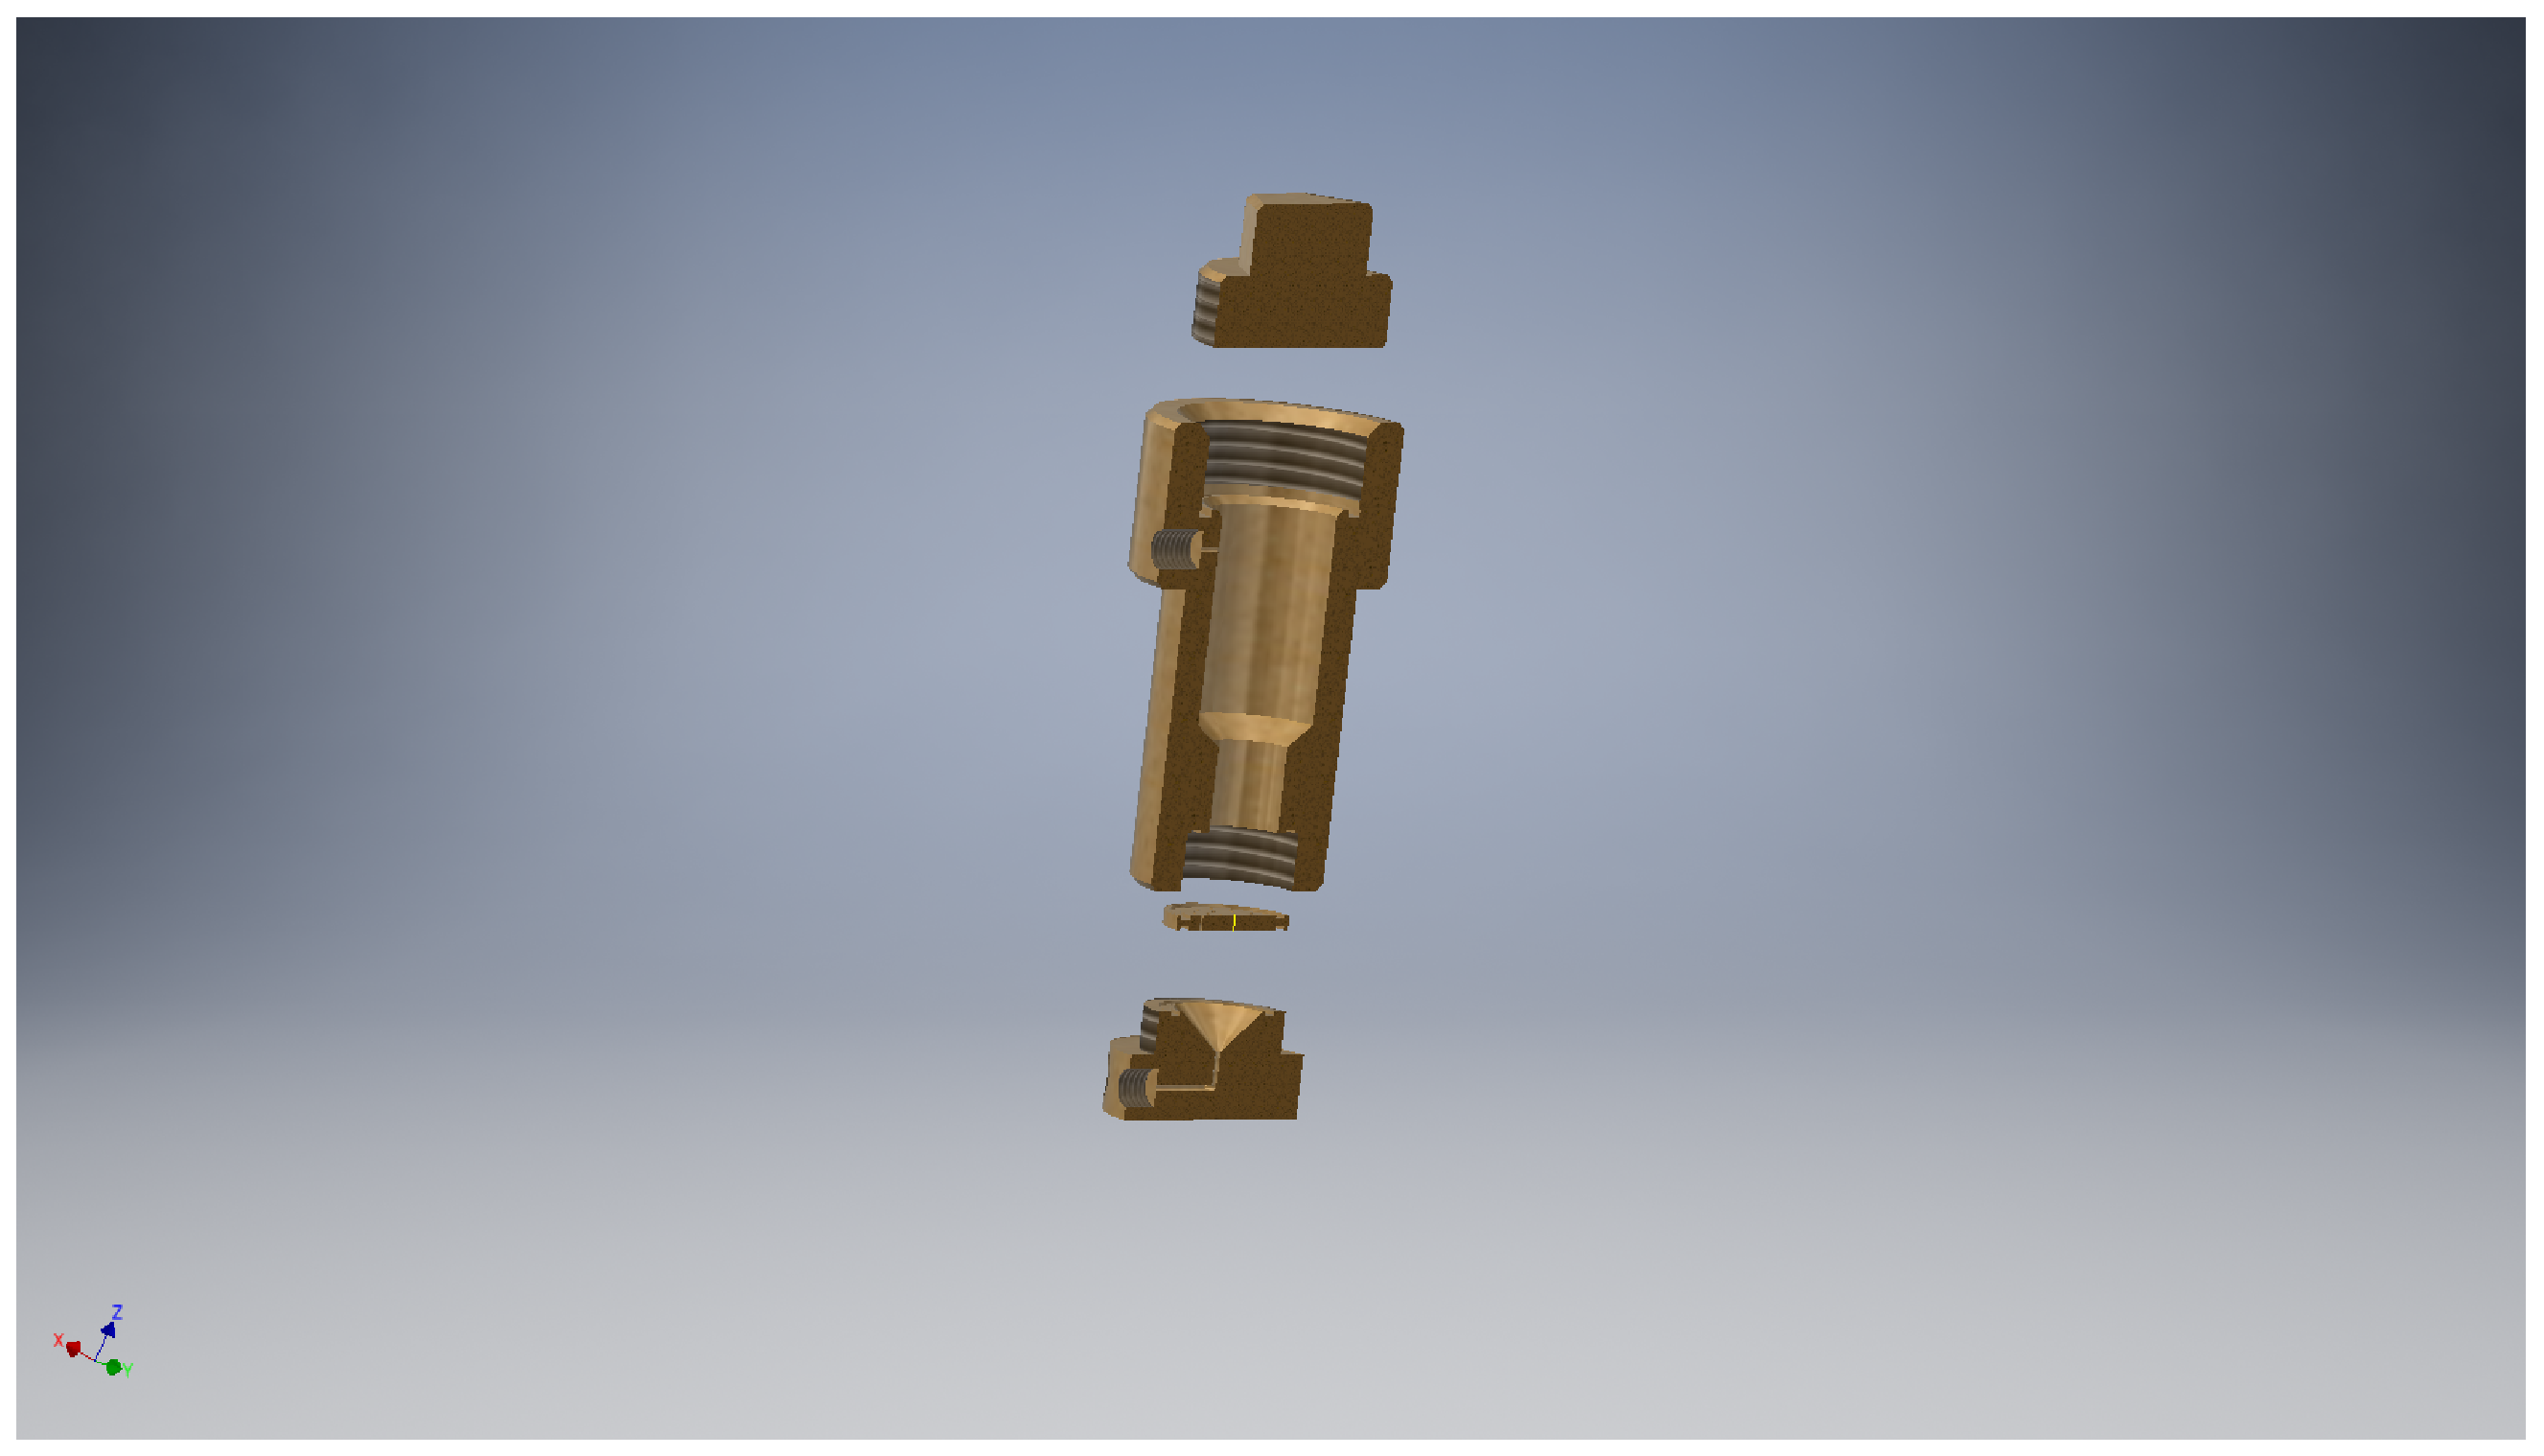
\includegraphics[width=0.49\textwidth]{/home/philipp/Documents/thesis/figures/materialsMethods/lowFieldReactor.eps}
				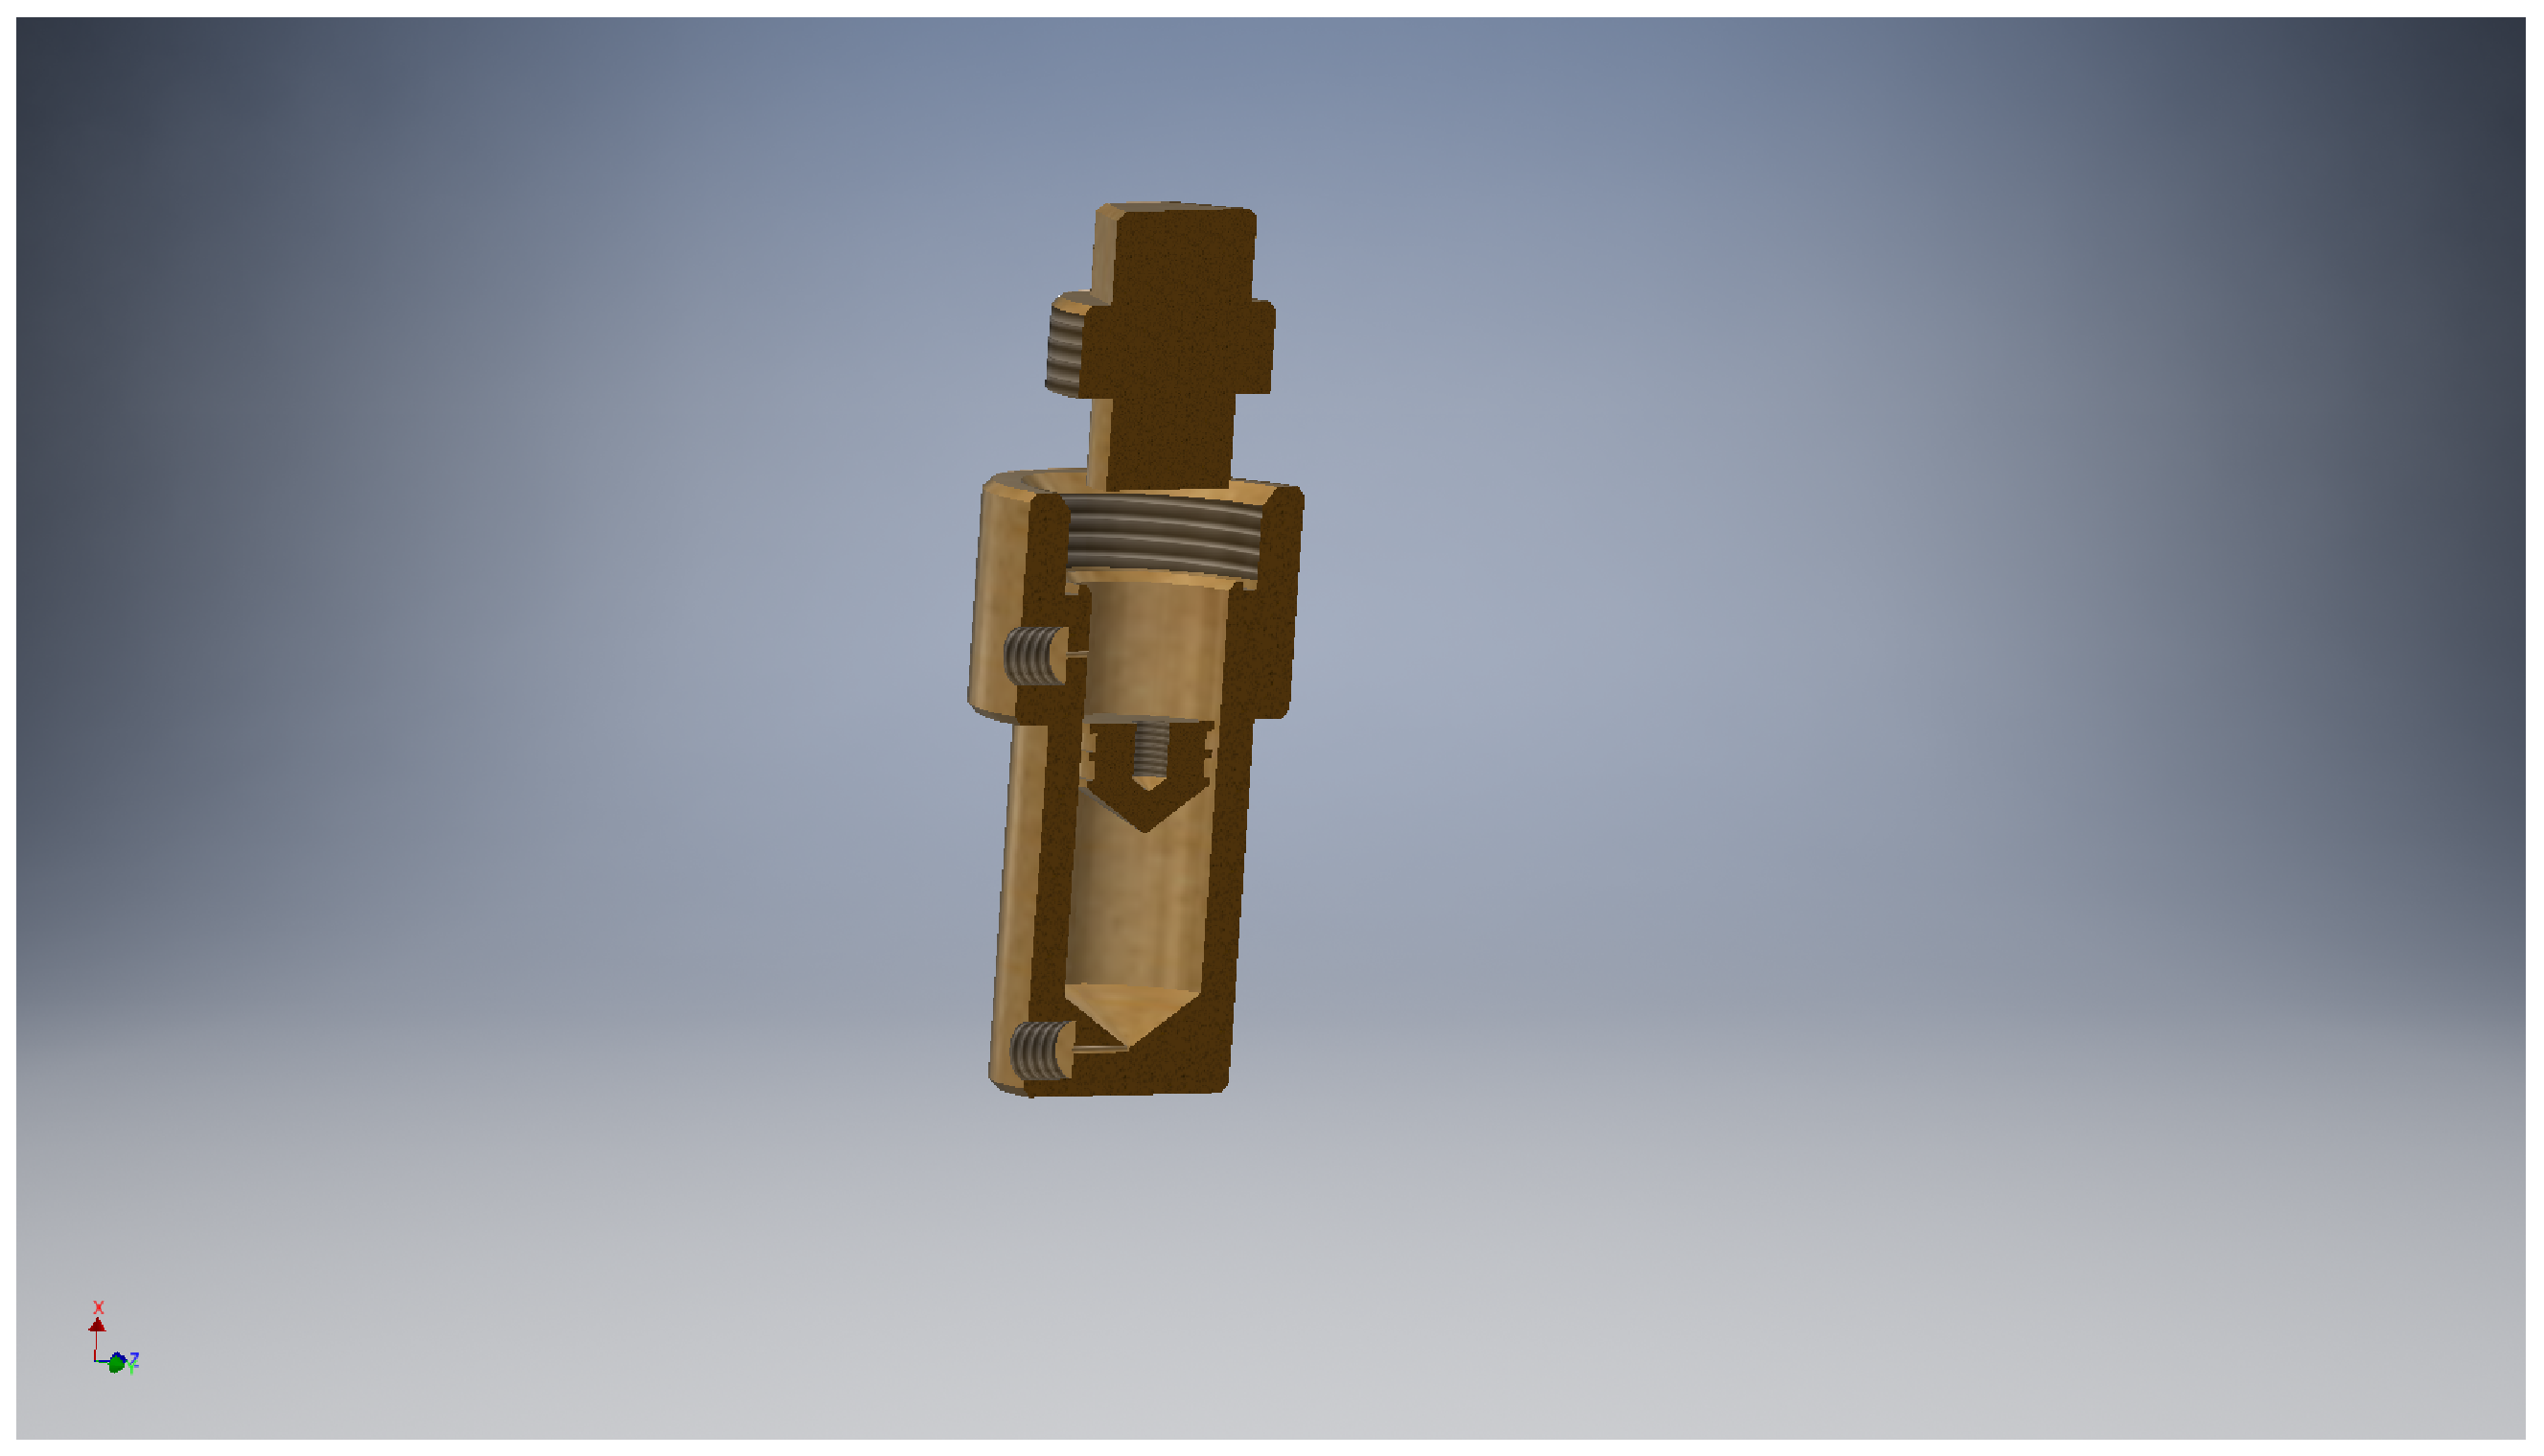
\includegraphics[width = 0.49 \textwidth]{/home/philipp/Documents/thesis/figures/materialsMethods/highFieldProbe.eps}
				\caption{Half cut views of the low field reactor (left) and high field probe
				(right). The disk for pH2 provision in the low field reactor is visisble on the bottom sandwiched between the
				main body and the screw on cap. Hose connections are made to that cap and the top
				of the main body. The high field probe is shown with its optional piston inserted,
				the two possible connections at the top for actuation and bottom for sample transfer
				are visible.}
			\end{figure}
		\subsection{High Field Probe}
			Similarly to the one in low field, the high field probe has to withstand the high
			pressures applied and the chemicals used. It is made from the same material, PSU. While
			its conical bottom is similar to the low field probe's, there's no need for a bubbling
			system. There are two procedures for shuttling the solution back to low field: Via a
			piston that can also be actuated by pressurized gas or simply by the gas pressure that
			builds above the solution due to the transfer towards high field. With methanol
			solutions, the latter method turns out to be efficient, other solutions with different
			viscosities may need the piston approach for efficient transport.
		\subsection{Fluid handling system} 
			Sample volumes range in the $\SI{}{\milli\litre}$ regime thus sample losses are
			unfavorable.
	\section{Fluxgate Field Probe}
		\subsection{Arduino Shield}
%\input{}
